% ============================================================
%  Chapitre 2 : Contexte et Problématique
%  Fichier : 05_context.tex
% ============================================================

\chapter{Contexte et Problématique}

La transformation numérique est devenue un impératif stratégique pour les
entreprises de toutes tailles et de tous secteurs. Selon IDC, les dépenses
mondiales en transformation digitale devraient atteindre près de
\textbf{4\,000 milliards USD d'ici 2027}, avec un taux de croissance annuel
composé (CAGR) de 16,2\,\%~\cite{integrate_io_stats}. Au cœur de cette
transformation se trouve un processus souvent sous-estimé mais fondamental :
la migration de données. Qu'il s'agisse de remplacer un système legacy par
une plateforme moderne, de consolider des bases de données après une
fusion-acquisition, d'adopter des solutions cloud pour gagner en agilité, ou
de préparer une infrastructure \textit{AI-ready} pour exploiter le potentiel
de l'intelligence artificielle, la migration constitue le socle invisible sur
lequel repose le succès --- ou l'échec --- de tout projet de modernisation.

Pourtant, la réalité est préoccupante : selon une analyse BCG portant sur
plus de 850 entreprises, seules \textbf{35\,\% des initiatives de
transformation digitale atteignent leurs objectifs}~\cite{integrate_io_stats}.
Le reste échoue ou livre des résultats en deçà des attentes, souvent à cause
de fondations de données fragiles. Ce chapitre dresse un panorama des enjeux
et des défis liés à la migration de données, avant de formuler la
problématique qui guidera l'ensemble de ce travail.

% ------------------------------------------------------------
\section{La migration de données : définition et enjeux}
% ------------------------------------------------------------

\subsection{Qu'est-ce qu'une migration de données ?}

La migration de données désigne le transfert structuré et planifié de données
d'un système source vers un système cible, en garantissant intégrité, qualité,
sécurité et conformité tout au long du processus. Ce processus repose sur le
triptyque \textbf{ETL} (\textit{Extract, Transform, Load})~\cite{microsoft_etl} :
extraction depuis le système source, transformation pour adapter les données au
modèle cible (nettoyage, standardisation, enrichissement, application des règles
métier), et chargement dans le nouveau système. Une variante moderne, l'approche
\textbf{ELT} (\textit{Extract, Load, Transform}), inverse les deux dernières
étapes en exploitant la puissance de calcul des entrepôts de données cloud
(Snowflake, BigQuery, Azure Synapse) pour effectuer les transformations après
le chargement~\cite{latentview2026, alphabyte_etl}.

\begin{figure}[H]
    \centering
    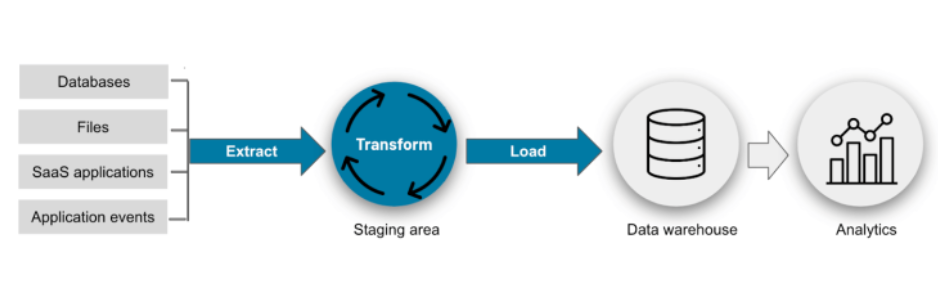
\includegraphics[width=0.85\linewidth]{img/ETL.png}
    \caption{Schéma du processus ETL classique --- extraction, transformation
    et chargement des données.}
    \label{fig:etl_schema}
\end{figure}

Il est important de distinguer la migration de données de concepts voisins :
l'\textbf{intégration continue} (synchronisation permanente entre systèmes
en temps réel), la \textbf{réplication} (copie à l'identique pour la haute
disponibilité) et l'\textbf{archivage} (déplacement de données historiques
vers un stockage de moindre coût). La migration se caractérise par son
caractère \textbf{ponctuel et planifié}, avec un périmètre défini, une
fenêtre d'exécution limitée et un objectif de basculement définitif vers
le système cible~\cite{cloudficient2025}.

Les projets de migration se déclinent en \textbf{cinq typologies
principales}~\cite{admp_core, latentview2026} :

\begin{itemize}
    \item \textbf{Re-platforming} --- Remplacement d'un système legacy par
    une plateforme moderne (Salesforce, SAP, Workday, Duck Creek). C'est le
    cas le plus fréquent dans le secteur de l'assurance et de la banque.

    \item \textbf{Consolidation post-fusion} --- Unification de bases de
    données hétérogènes suite à une fusion-acquisition, nécessitant la
    réconciliation de schémas, de référentiels et de règles métier
    divergents.

    \item \textbf{Migration cloud} --- Transfert des données et des
    workloads vers des plateformes cloud (AWS, Azure, GCP). En 2026,
    \textbf{94\,\% des entreprises} utilisent au moins un service cloud
    et \textbf{60\,\% des données d'entreprise} sont désormais stockées
    dans le cloud~\cite{medhacloud2026, datastackhub2026}.

    \item \textbf{Profiling et cleansing} --- Amélioration de la qualité
    des données (dédoublonnage, normalisation, enrichissement) avant
    réinjection dans le système existant ou un nouveau système.

    \item \textbf{Externalisation BPO} --- Transfert sécurisé de données
    vers un prestataire externe dans le cadre d'une externalisation de
    processus métier.
\end{itemize}

\subsection{Enjeux stratégiques pour les entreprises}

La migration de données est bien plus qu'un exercice technique : c'est un
enjeu stratégique à fort impact business dont les dimensions sont multiples.

\subsubsection{Un marché en croissance exponentielle}

Le marché mondial de la migration de données connaît une expansion
remarquable. Selon les estimations convergentes de plusieurs cabinets
d'analyse, il est évalué entre \textbf{15 et 21 milliards USD en 2025}
et devrait atteindre \textbf{36 à 48 milliards USD d'ici 2032--2035},
avec un CAGR oscillant entre 12 et 17\,\% selon les
périmètres~\cite{datamintel2026, reportsanddata2026, researchandmarkets2026,
fortunebi2026}. Le marché plus large des services de migration cloud
représente à lui seul \textbf{31,5 milliards USD en 2026}, avec un CAGR
de 22,4\,\%~\cite{medhacloud2026}.

\begin{figure}[H]
    \centering
    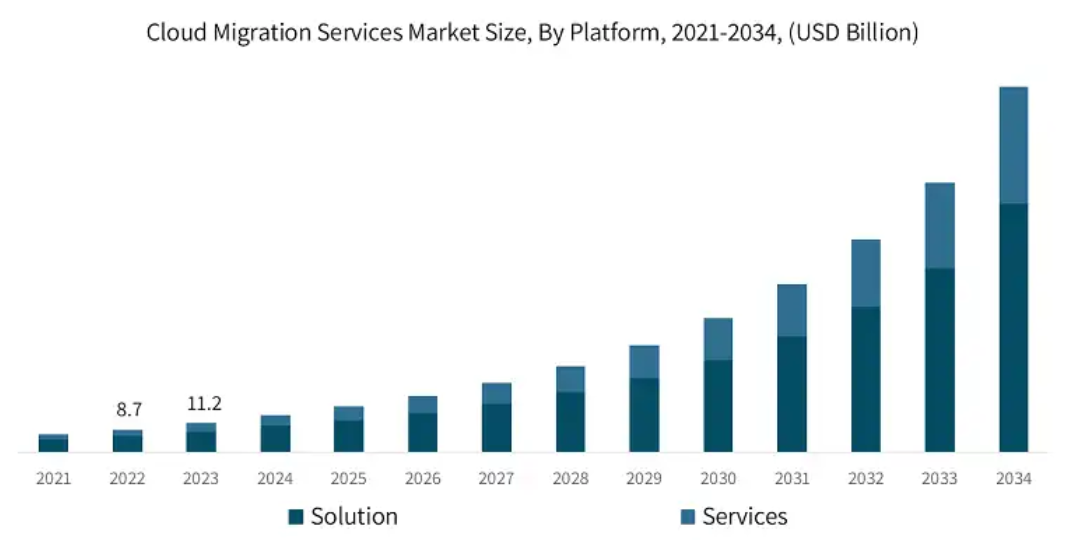
\includegraphics[width=0.85\linewidth]{img/migration_prev.png}
    \caption{Évolution du marché mondial de la migration de données
    (2024--2035), sources multiples.}
    \label{fig:market_growth}
\end{figure}

Cette croissance est portée par quatre forces motrices majeures identifiées
par Business Research Insights~\cite{bri2026} : l'\textbf{adoption du cloud}
(facteur cité par 65\,\% des organisations), la \textbf{croissance des volumes
de données} (58\,\%), les \textbf{initiatives de transformation digitale}
(62\,\%) et l'\textbf{adoption de l'IA et de l'automatisation} (54\,\%).

\subsubsection{Les dimensions stratégiques de la migration}

Tu peux la condenser ainsi :

Au-delà de la croissance du marché, plusieurs enjeux stratégiques rendent la migration des données essentielle. Elle garantit la continuité d’activité en limitant les risques de perte de données, assure la conformité réglementaire face aux exigences croissantes de protection des données, et représente un enjeu majeur de maîtrise des coûts dans les projets de modernisation IT. Elle constitue également une base indispensable pour les initiatives d’IA et d’analytique avancée, qui reposent sur des données fiables et bien gouvernées. Enfin, une migration réussie procure un avantage concurrentiel, en permettant aux entreprises d’exploiter leurs données plus rapidement et d’améliorer leur retour sur investissement.


% ------------------------------------------------------------
\section{Anatomie d'un projet de migration : les défis}
% ------------------------------------------------------------

Malgré son importance stratégique, la migration de données reste l'un des
processus les plus risqués du paysage IT. Les statistiques sont éloquentes :
selon Gartner, \textbf{83\,\% des projets de migration échouent ou dépassent
leur budget et leurs délais}~\cite{kaopiz2025, kanerika2025}. Le Bloor Group
rapporte des dépassements moyens de \textbf{30\,\% en coût et de 41\,\% en
délai}~\cite{vovance_medium}. Et selon les données Accenture les plus
récentes, seules \textbf{65\,\% des migrations sont livrées dans les temps
et le budget prévu}~\cite{medhacloud2026}. Six défis structurels expliquent
ces résultats.

\begin{figure}[H]
    \centering
    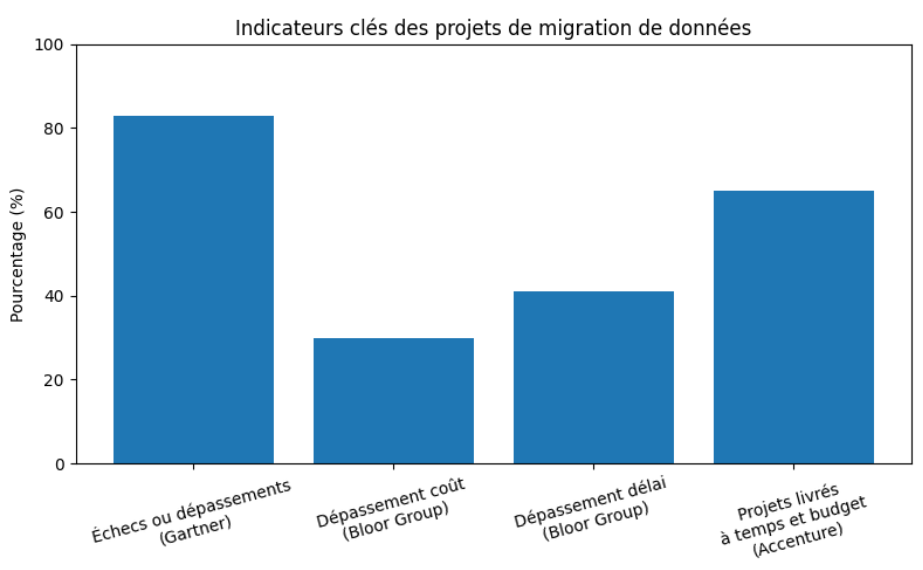
\includegraphics[width=0.85\linewidth]{img/graphe.png}
    \caption{les défis d'un projet de migration}
    \label{fig:market_growth}
\end{figure}

\subsection{Hétérogénéité des systèmes source et cible}

Le premier défi fondamental réside dans la disparité entre les systèmes
d'origine et de destination. Les données sources peuvent provenir de bases
relationnelles (Oracle, SQL Server, DB2), de fichiers plats (CSV, TXT), de
systèmes mainframe (VSAM, IMS), ou d'applications métier propriétaires,
chacun avec ses propres formats, encodages et conventions de
nommage~\cite{admp_presentation}. Le système cible, quant à lui, impose
son propre modèle de données, ses contraintes d'intégrité référentielle et
ses règles de validation.

Cette hétérogénéité génère des incompatibilités de schéma à l'origine de
\textbf{45\,\% des échecs de migration}~\cite{cloudficient2025}. La
réconciliation entre ces modèles divergents nécessite un travail minutieux
de mapping --- à la fois au niveau des tables (\textit{Table Mapping}) et
des champs (\textit{Data Mapping}) --- qui constitue l'un des exercices les
plus chronophages et les plus sujets à erreur. Un exemple révélateur : un
assureur majeur a vu 127\,000 polices des années 1940 migrées avec une date
d'émission en 2040, en raison d'un bug non documenté de format de dates dans
le système legacy~\cite{vovance_medium}.

\subsection{Volumétrie et performance}
La part des workloads d’entreprise déployés dans des environnements cloud ou edge devrait connaître une forte progression au cours des prochaines années. Selon Gartner, cette proportion passera de 52  en 2024 à 75  en 2028, soit une augmentation de 23 points en quatre ans. Cette évolution traduit l’accélération de la transformation numérique et entraîne des migrations de données de plus en plus massives. Les entreprises doivent ainsi gérer des volumes croissants de données tout en faisant face à des contraintes de bande passante, de latence et de disponibilité, ce qui accroît considérablement la complexité de la planification et de l’exécution des migrations.

\begin{figure}[H]
    \centering
    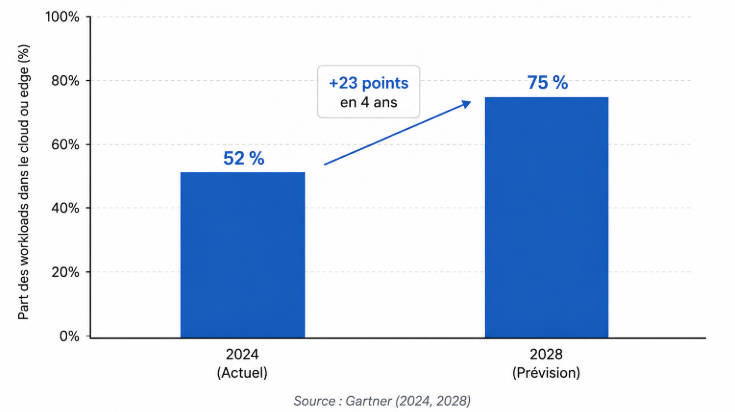
\includegraphics[width=0.85\linewidth]{img/graphe1.png}
    \caption{Evolution de la part des woekloads d'entreprise dans des environnements cloud ou edge}
    \label{fig:market_growth}
\end{figure}

~\cite{kaopiz2025}
~\cite{medhacloud2026}

\subsection{Qualité et intégrité des données}

La mauvaise qualité des données représente un risque financier et opérationnel majeur,
dont l'impact est particulièrement exacerbé lors des phases de migration.Ce phénomène engendre des coûts micro et macroéconomiques colossaux, tout en altérant structurellement la réussite des projets.

En contexte de migration, ces défaillances (données incomplètes, dupliquées ou corrompues) 
deviennent le principal facteur de dérive des projets. Elles se traduisent par des retards 
systématiques pour près de la moitié des organisations, provoquant par effet de cascade une explosion des budgets et un taux d'échec critique sur les délais de livraison.

~\cite{gartner_quality}
~\cite{forbes_bad_data}.
~\cite{alation_migration}. 
~\cite{montecarlo2025}.

\begin{figure}[H]
    \centering
    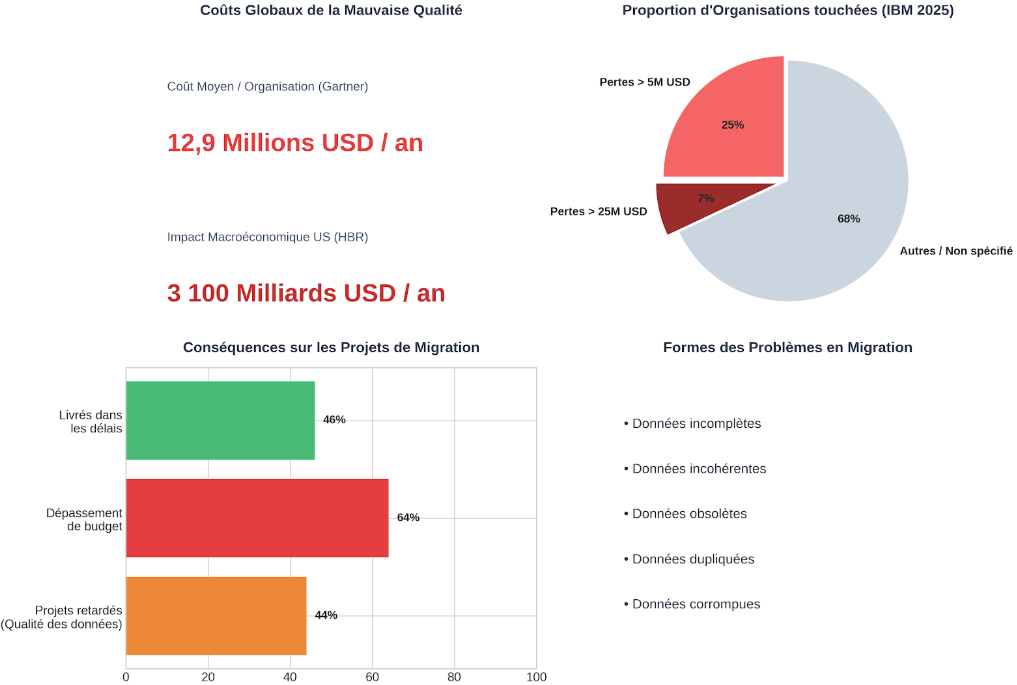
\includegraphics[width=0.85\linewidth]{img/impact_data_quality.png}
    \caption{L'impact de la mauvaise qualité des données}
    \label{fig:market_growth}
\end{figure}

\subsection{Complexité des règles de transformation}

La migration ne se limite pas à un simple transfert de données : elle
implique l'application de règles métier souvent complexes et mal
documentées. Parmi les défis typiques :

\begin{itemize}
    \item Relations \textbf{N:M} entre tables source et cible, nécessitant
    des mécanismes de dédoublonnage et de réconciliation.
    \item \textbf{Transcodification} entre référentiels source et cible
    (codes produits, statuts, identifiants).
    \item \textbf{Création conditionnelle} d'enregistrements selon des
    critères métier (périmètre fonctionnel, scope de migration).
    \item Gestion des \textbf{cas particuliers} et des données historiques
    (polices résiliées, bénéficiaires décédés, dossiers archivés).
    \item \textbf{Logique de fallback} lorsque des données source sont
    absentes ou invalides.
\end{itemize}

La formalisation de ces règles constitue l'un des postes les plus coûteux en
temps et en expertise, creusant le fossé entre spécifications fonctionnelles
et traduction technique. Comme le souligne Kanerika, les pipelines ETL
\textbf{encodent de la logique métier} : une seule règle mal traduite peut
corrompre des rapports financiers pendant des mois avant d'être
détectée~\cite{kanerika_etl}.

\subsection{Traçabilité et auditabilité}

Dans un environnement réglementaire de plus en plus exigeant,
\textbf{34\,\% des organisations rapportent des lacunes de conformité
durant la migration} et \textbf{38\,\% déclarent que la préparation aux
audits est difficile}~\cite{gitnux_cloud, admp_overview}. Les outils ETL
traditionnels, souvent qualifiés de \textbf{boîtes noires} (\textit{black
boxes}), rendent cette traçabilité particulièrement ardue : les
transformations appliquées aux données sont opaques, les versions des règles
difficiles à suivre, et la réconciliation entre données source et cible
laborieuse.

Cette opacité est d'autant plus problématique que les organisations doivent
aujourd'hui garantir une \textbf{traçabilité de bout en bout}
(\textit{data lineage}) de chaque donnée migrée, depuis son extraction du
système source jusqu'à son chargement dans le système cible, en passant par
chaque transformation appliquée. Les régulateurs exigent de pouvoir auditer
chaque étape du processus, ce qui impose des mécanismes de versionnement,
de journalisation et de reporting que les approches traditionnelles peinent
à fournir.

\subsection{Coordination IT / Business et gestion du changement}

La migration se situe à l'intersection des équipes techniques et métier,
générant une véritable \textbf{barrière linguistique} entre ces deux
mondes. Les spécificateurs fonctionnels décrivent des règles métier en
langage naturel, tandis que les développeurs doivent les traduire en code
technique --- un processus source d'erreurs d'interprétation, de cycles de
validation longs et de frustrations mutuelles.

Les statistiques confirment l'ampleur du problème : \textbf{70\,\% des
migrations échouent en partie à cause d'une mauvaise gestion du changement},
et \textbf{80\,\% des organisations citent le manque d'expertise interne
comme principal frein}~\cite{worldmetrics2025, wifitalents2025}. La pénurie
de talents IT est critique : selon les projections, jusqu'à \textbf{90\,\%
des organisations feront face à des pénuries de compétences IT}, avec des
pertes estimées à \textbf{5\,500 milliards USD d'ici 2026} liées à ces
lacunes~\cite{integrate_io_stats}.

De plus, la résistance au changement des utilisateurs finaux, combinée à
une formation insuffisante, compromet l'adoption du nouveau système même
lorsque la migration technique est réussie. Dans le domaine des ERP, par
exemple, \textbf{29\,\% des utilisateurs} déclarent ne pas comprendre
comment utiliser le nouveau système après migration~\cite{godlan_erp}.

\begin{table}[H]
\centering
\caption{Synthèse des principaux défis d'un projet de migration de données.}
\label{tab:defis_migration}
\begin{tabular}{lll}
\hline
\textbf{Défi} & \textbf{Impact principal} & \textbf{Statistique clé} \\
\hline
Hétérogénéité des systèmes    & Incompatibilités, corruption   & 45\,\% des échecs \\
Volumétrie et performance     & Dépassements de délais         & 181 ZB créés en 2025 \\
Qualité des données           & Surcoûts, reprises             & 12,9 M\$/an (Gartner) \\
Complexité des transformations & Écart design--build           & 30--50\,\% du budget IT \\
Traçabilité et auditabilité   & Non-conformité                 & 34\,\% de lacunes \\
Coordination IT / Business    & Retards, malentendus           & 70\,\% liés au change management \\
\hline
\end{tabular}
\end{table}

% ------------------------------------------------------------
\section{L'émergence de l'IA dans la migration de données}
% ------------------------------------------------------------

Face à ces défis, l'intelligence artificielle émerge comme un levier
transformateur. Selon Business Research Insights: 

\begin{figure}[H]
    \centering
    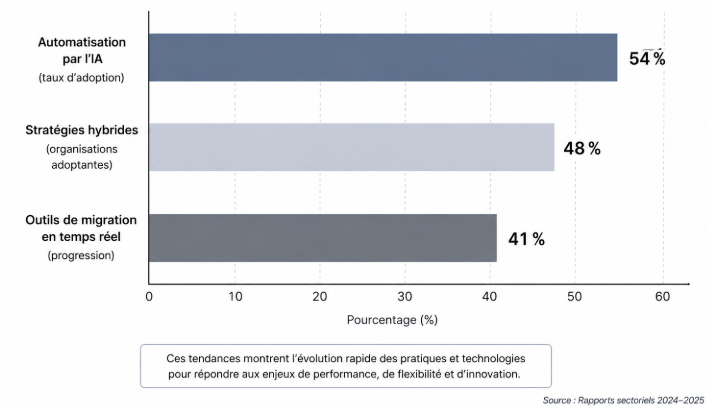
\includegraphics[width=0.85\linewidth]{img/graphe2.png}
    \caption{Tendances clés dans les solutions de migration}
    \label{fig:market_growth}
\end{figure}

~\cite{bri2026}.

L'IA transforme la migration de données à plusieurs niveaux~\cite{buzzclan2026,
ispirer_ai} :

\begin{itemize}
    \item \textbf{Data profiling intelligent} : Les algorithmes de ML
    détectent automatiquement les anomalies, les valeurs nulles dans des
    colonnes inattendues, les formats de dates non documentés et les
    enregistrements orphelins, là où le profiling manuel procède par
    échantillonnage statistique.

    \item \textbf{Mapping automatisé} : L'IA analyse les systèmes source
    et cible pour créer des correspondances de schéma sans intervention
    manuelle, réduisant drastiquement le temps de mapping.

    \item \textbf{Validation prédictive} : Les modèles de ML identifient
    les goulots d'étranglement et les risques de défaillance avant qu'ils
    ne surviennent, permettant une approche proactive plutôt que réactive.

    \item \textbf{Génération de règles de transformation} : Les LLM
    (\textit{Large Language Models}) peuvent générer des règles de
    transformation à partir de spécifications en langage naturel, comblant
    le fossé entre spécificateurs fonctionnels et développeurs.

    \item \textbf{Optimisation des coûts} : L'IA identifie les données
    redondantes ou non critiques, réduisant les volumes à migrer et les
    coûts de stockage associés.
\end{itemize}

Selon les projections, l'IA augmentée en gestion de données pourrait
\textbf{réduire de 45\,\% le besoin en spécialistes IT} pour les tâches
routinières de migration~\cite{ispirer_ai}. Cependant, malgré ces promesses,
l'adoption reste limitée : seulement \textbf{35\,\% des entreprises}
utilisent actuellement des plateformes de migration augmentées par
l'IA~\cite{reanin2025}, et \textbf{74\,\% des entreprises peinent à
passer à l'échelle} avec leurs initiatives IA~\cite{integrate_io_stats}.
Cet écart entre potentiel et adoption constitue une opportunité majeure
pour les acteurs innovants du marché.

% ------------------------------------------------------------
\section{Formulation de la problématique}
% ------------------------------------------------------------

L'analyse précédente fait émerger trois lacunes structurelles communes aux
approches actuelles de migration, que nous synthétisons dans la figure
ci-dessous :

\begin{itemize}
 \item \textbf{Le fossé Design-Build} : un décalage significatif persiste
entre la rédaction des spécifications fonctionnelles et leur implémentation
technique. Les spécificateurs décrivent les règles métier en langage naturel,
les développeurs les traduisent en code, et entre les deux, la perte de
fidélité est inévitable~\cite{admp_overview}. Ce fossé ne se limite d'ailleurs
pas au code applicatif : la traduction doit aboutir à des artefacts
d'intégration réellement exécutables sur les plateformes cloud d'orchestration
(par exemple des pipelines Azure Data Factory), ce qui ajoute une couche
d'expertise technique et autant de sources d'erreur.

    \item \textbf{L'opacité des processus} : les outils ETL traditionnels
    fonctionnent comme des boîtes noires, rendant difficile la validation
    fonctionnelle, l'auditabilité et la réconciliation par les équipes non
    techniques. Dans un contexte réglementaire où 172 pays disposent de lois
    sur la protection des données~\cite{stationx_privacy}, cette opacité
    n'est plus acceptable.

    \item \textbf{L'absence d'intelligence artificielle} : les processus de
    migration restent largement manuels et réactifs, alors que l'IA offre
    des possibilités transformatrices en matière d'automatisation, de
    validation prédictive et de génération intelligente de règles.
    Seulement \textbf{35\,\% des entreprises} utilisent des plateformes
    augmentées par l'IA~\cite{reanin2025}, laissant un immense potentiel
    inexploité.
\end{itemize}

Ces constats, croisés avec les réalités du terrain observées dans le cadre
de ce stage au sein de l'équipe ADMP d'Accenture, amènent à formuler la
problématique suivante :

\begin{quote}
\textit{Comment concevoir et implémenter une plateforme de migration de
données intégrant l'intelligence artificielle pour automatiser et optimiser
les processus d'intégration, réduire le fossé entre la conception
fonctionnelle et l'exécution technique, et améliorer la qualité, la
traçabilité et l'efficience globale du processus de migration ?}
\end{quote}

Cette problématique sera explorée à travers l'état de l'art (chapitre
suivant), qui examinera les solutions existantes  y compris la plateforme
ADMP et son architecture actuelle  et les avancées de l'IA dans ce
domaine, avant de présenter notre contribution : le développement d'un
module de génération automatisée intégré à l'évolution IA de la plateforme
ADMP.